\documentclass[12pt,a4paper,oneside]{article}

%--------------------------- Codificacao e idioma ---------------------
\usepackage[T1]{fontenc}
\usepackage[utf8]{inputenc}
% No Overleaf o babel em portugues esta disponivel; o teste abaixo apenas
% evita erro em instalacoes minimas do TeX sem o pacote de idioma.
\IfFileExists{portuges.ldf}{\usepackage[brazil]{babel}}{%
  \renewcommand{\contentsname}{Sumário}
  \renewcommand{\refname}{Referências}
  \renewcommand{\figurename}{Figura}
  \renewcommand{\tablename}{Tabela}
  \renewcommand{\appendixname}{Apêndice}
  \renewcommand{\abstractname}{Resumo}}

%--------------------------- Fonte e margens (ABNT) -------------------
\usepackage{mathptmx}
\usepackage[a4paper,left=3cm,right=2cm,top=3cm,bottom=2cm]{geometry}

%--------------------------- Pacotes -----------------------------------
\usepackage{amsmath,amssymb}
\usepackage{graphicx}
\usepackage{setspace}       % requerido pela capa
\usepackage{ragged2e}       % requerido pela capa
\usepackage{indentfirst}
\usepackage{booktabs}
\usepackage{xcolor}
\usepackage{float}
\usepackage{caption}
\usepackage{subcaption}
\usepackage{fancyhdr}
\usepackage{listings}
\usepackage{microtype}
\usepackage[hidelinks]{hyperref}

\captionsetup{font=small,labelfont=bf,labelsep=endash}
\graphicspath{{figuras/}}

%--------------------------- Parametros gerais -------------------------
\onehalfspacing
\setlength{\parindent}{1.25cm}
\setlength{\headheight}{15pt}
\pagestyle{fancy}
\fancyhf{}
\renewcommand{\headrulewidth}{0pt}
\fancyhead[R]{\small\thepage}

\lstset{
  language=Python, basicstyle=\ttfamily\scriptsize, columns=fullflexible,
  keywordstyle=\color{blue!60!black}\bfseries,
  commentstyle=\color{green!35!black}\itshape,
  stringstyle=\color{orange!60!black},
  numbers=left, numberstyle=\tiny\color{gray}, frame=single,
  breaklines=true, showstringspaces=false, tabsize=4,
  extendedchars=true,
  literate={á}{{\'a}}1 {é}{{\'e}}1 {É}{{\'E}}1 {ç}{{\c{c}}}1 {ã}{{\~a}}1
}

\newcommand{\EQ}{\mathrm{EQ}}

%--------------------------- Capa e folha de rosto ---------------------
%=====================================================================
%  BLOCO REUTILIZAVEL: CAPA + FOLHA DE ROSTO (ABNT NBR 14724)
%  Modelo do autor (PPGEELT/UFU). Requer no preambulo principal:
%  graphicx, setspace e ragged2e.
%  Os campos podem ser redefinidos com \renewcommand apos o \input.
%=====================================================================

%--------------------------- Logos opcionais --------------------------
\newcommand{\logoou}[2]{%
  \IfFileExists{#1}{\includegraphics[height=#2,width=\linewidth,keepaspectratio]{#1}}%
                   {\rule{0pt}{#2}}}

%=====================================================================
%  >>>>>>>>>>>>>>  PREENCHA AQUI OS DADOS DO TRABALHO  <<<<<<<<<<<<<<
%=====================================================================
\newcommand{\vazio}{}   % marcador interno para campos opcionais -- nao altere

\newcommand{\Autor}{LUCAS ALBINO MARTINS}
\newcommand{\Titulo}{Trabalho 09 - Mapas Auto-Organiz\'aveis de Kohonen}
\newcommand{\Subtitulo}{Disciplina: EL056 - Redes Neurais Artificiais}
\newcommand{\Orientador}{Prof. Dr. Keiji Yamanaka}
\newcommand{\Coorientador}{}                    % vazio se nao houver
\newcommand{\Matricula}{12622EEL006}            % vazio para omitir
\newcommand{\Local}{Uberl\^andia}
\newcommand{\Ano}{2026}

% ---- Titulo do elemento textual (cabecalho da 1a pagina de texto) ----
\newcommand{\TituloTexto}{Mapa auto-organiz\'avel de Kohonen com topologia linear}

% ---- Nota de apresentacao da folha de rosto --------------------------
\newcommand{\NotaApresentacao}{%
  Trabalho apresentado ao Programa de P\'os-Gradua\c{c}\~ao em Engenharia
  El\'etrica (PPGEELT) da Universidade Federal de Uberl\^andia como
  requisito parcial de avalia\c{c}\~ao da disciplina.

  \vspace{0.45cm}
  Disciplina: EL056 - Redes Neurais Artificiais.

  \vspace{0.45cm}
  Professor: \Orientador.
  \ifx\Coorientador\vazio\else

    \vspace{0.2cm}
    Coorientador: \Coorientador.
  \fi
}

%--------------------- Logos (troque pelos arquivos reais) ------------
\newcommand{\LogoEsquerda}{logos/logo-ppgeel.png}
\newcommand{\LogoDireita}{logos/logo-ufu.png}
\newcommand{\AlturaLogoEsq}{2.2cm}   % ajuste fino da altura de cada logo
\newcommand{\AlturaLogoDir}{2.6cm}

%=====================================================================
%  CABECALHO INSTITUCIONAL (logos + nome da instituicao + filete)
%=====================================================================
\newcommand{\cabecalhoinstitucional}{%
  \begin{center}
    \noindent
    \begin{minipage}[c]{0.19\textwidth}
      \raggedright
      \logoou{\LogoEsquerda}{\AlturaLogoEsq}
    \end{minipage}%
    \hfill
    \begin{minipage}[c]{0.58\textwidth}
      \centering
      \singlespacing
      {\fontsize{12}{15}\selectfont\bfseries
        UNIVERSIDADE FEDERAL DE UBERL\^ANDIA\par}
      \vspace{0.25cm}
      {\fontsize{12}{15}\selectfont
        PPGEELT -- P\'os-Gradua\c{c}\~ao em Engenharia El\'etrica\par}
    \end{minipage}%
    \hfill
    \begin{minipage}[c]{0.19\textwidth}
      \raggedleft
      \logoou{\LogoDireita}{\AlturaLogoDir}
    \end{minipage}

    \vspace{0.35cm}
    \rule{\textwidth}{1.1pt}
  \end{center}
}

%=====================================================================
%  CAPA -- ABNT NBR 14724
%=====================================================================
\newcommand{\fazcapa}{%
  \thispagestyle{empty}
  \begin{center}
    \cabecalhoinstitucional

    \vspace{2.5cm}

    {\fontsize{12}{15}\selectfont\MakeUppercase{\Autor}\par}

    \ifx\Matricula\vazio\else
      \vspace{0.4cm}
      {\fontsize{11}{14}\selectfont Matr\'icula: \Matricula\par}
    \fi

    \vspace{4.0cm}

    {\fontsize{16}{20}\selectfont\bfseries\MakeUppercase{\Titulo}\par}
    \ifx\Subtitulo\vazio\else
      \vspace{0.35cm}
      {\fontsize{13}{16}\selectfont\Subtitulo\par}
    \fi

    \vfill

    {\fontsize{12}{15}\selectfont \Local\par}
    \vspace{0.15cm}
    {\fontsize{12}{15}\selectfont \Ano\par}
  \end{center}
  \newpage
  \setcounter{page}{1}   % a contagem ABNT comeca na folha de rosto
}

%=====================================================================
%  FOLHA DE ROSTO -- ABNT NBR 14724
%=====================================================================
\newcommand{\fazfolhaderosto}{%
  \thispagestyle{empty}
  \begin{center}
    \cabecalhoinstitucional

    \vspace{2.0cm}

    {\fontsize{12}{15}\selectfont\MakeUppercase{\Autor}\par}

    \vspace{3.0cm}

    {\fontsize{16}{20}\selectfont\bfseries\MakeUppercase{\Titulo}\par}
    \ifx\Subtitulo\vazio\else
      \vspace{0.35cm}
      {\fontsize{13}{16}\selectfont\Subtitulo\par}
    \fi
  \end{center}

  \vspace{2.0cm}

  \hfill
  \begin{minipage}{0.5\textwidth}
    \singlespacing
    \setlength{\parindent}{0pt}
    \fontsize{10}{12}\selectfont
    \justifying
    \NotaApresentacao
  \end{minipage}

  \vfill

  \begin{center}
    {\fontsize{12}{15}\selectfont \Local\par}
    \vspace{0.15cm}
    {\fontsize{12}{15}\selectfont \Ano\par}
  \end{center}
  \newpage
}


\begin{document}

\fazcapa
\fazfolhaderosto

\begin{center}
  {\bfseries\MakeUppercase{\TituloTexto}}
\end{center}

\begin{abstract}
\noindent Este trabalho resolve o Exercício 4.1 de Fausett (1994):
uma rede de Kohonen com duas entradas e 50 unidades de cluster dispostas em
linha é treinada com 100 pontos uniformemente distribuídos no disco
$x_1^2+x_2^2<0{,}25$, usando vizinhança fixa de raio $R=1$ e taxa de
aprendizado decrescendo linearmente de $0{,}5$ a $0{,}01$ em 100 épocas.
A implementação foi feita em Python e NumPy, sem bibliotecas de SOM prontas.
Em dez épocas o emaranhado aleatório inicial (209 cruzamentos da cadeia) é
recolhido para dentro do disco e a cadeia de pesos passa a serpentear pela
região dos dados; o erro de quantização médio cai de $0{,}140$ para $0{,}042$.
Com $R=1$ fixo, porém, restam alguns cruzamentos (``nós'') que a rede não
consegue desfazer. Análises complementares mostram que o tipo de decaimento
de $\alpha$ pouco altera o resultado, que a quantidade de nós depende da
inicialização e que um raio inicial grande elimina os nós por completo.

\medskip
\noindent\textbf{Palavras-chave:} mapas auto-organizáveis; Kohonen;
aprendizado competitivo; preservação topológica.
\end{abstract}

%=====================================================================
\section{Introdução}
%=====================================================================

Os mapas auto-organizáveis (\textit{Self-Organizing Maps}, SOM), propostos
por Kohonen (1982), são redes de aprendizado \emph{competitivo} e
\emph{não supervisionado}. As unidades de saída (unidades de cluster) estão
arranjadas segundo uma topologia fixa, como uma linha ou uma grade, e cada
uma possui um vetor de pesos com a mesma dimensão das entradas. Quando um
padrão $\mathbf{x}$ é apresentado, as unidades competem: vence aquela cujo
vetor de pesos está mais próximo de $\mathbf{x}$. Diferentemente do
aprendizado competitivo puro (``o vencedor leva tudo''), no SOM o vencedor e
seus \emph{vizinhos topológicos} são deslocados na direção do padrão
(FAUSETT, 1994; HAYKIN, 2001).

Essa cooperação local é o mecanismo da \emph{preservação topológica}:
unidades vizinhas na grade de saída são repetidamente arrastadas para as
mesmas regiões do espaço de entrada e, ao fim do treino, passam a representar
regiões vizinhas. O mapa resultante é uma projeção ordenada do espaço de
entrada sobre a topologia de saída (KOHONEN, 2001). Quando a topologia é
linear e a entrada é bidimensional, a rede precisa ``costurar'' uma curva
unidimensional pela região dos dados, algo próximo de uma curva que preenche
o plano. Essa é a situação do Exercício 4.1, e permite visualizar
diretamente, no plano $(w_1,w_2)$, o processo de auto-organização.

%=====================================================================
\section{Metodologia}
%=====================================================================

\subsection{Arquitetura e algoritmo}

A rede tem $n=2$ unidades de entrada e $m=50$ unidades de cluster
$C_1,\dots,C_{50}$ em topologia linear. O vetor de pesos da unidade $C_j$ é
$\mathbf{w}_{\cdot j}=(w_{1j},w_{2j})$, inicializado com componentes
independentes $w_{ij}\sim U(-1,1)$. Para cada padrão $\mathbf{x}$:

\begin{enumerate}
  \item \textbf{Competição:} calcula-se
  $D(j)=\sum_{i=1}^{2}(w_{ij}-x_i)^2$ para $j=1,\dots,50$, e o vencedor é
  $J=\arg\min_j D(j)$.
  \item \textbf{Cooperação:} a vizinhança de raio $R=1$ é
  $\mathcal{N}(J)=\{J-1,\,J,\,J+1\}\cap\{1,\dots,50\}$; nas bordas o vizinho
  inexistente é simplesmente ignorado, de modo que $C_1$ e $C_{50}$ têm um
  único vizinho.
  \item \textbf{Adaptação:} para todo $j\in\mathcal{N}(J)$,
  \begin{equation}
    w_{ij}(\text{novo}) = w_{ij}(\text{velho})
      + \alpha\,\bigl[x_i - w_{ij}(\text{velho})\bigr].
    \label{eq:atualizacao}
  \end{equation}
\end{enumerate}

Uma época consiste na apresentação dos 100 padrões em ordem aleatória,
sorteada novamente a cada época. O raio $R=1$ permanece fixo durante todo o
treino, e o treinamento dura 100 épocas.

\subsection{Geração dos dados}

Os 100 pontos de treino foram obtidos por amostragem por rejeição: sorteiam-se
$x_1,x_2\sim U(-0{,}5;\,0{,}5)$ e o ponto é aceito somente se
$x_1^2+x_2^2<0{,}25$. O processo se repete até haver 100 pontos aceitos, o
que resulta em uma distribuição uniforme no disco de raio $0{,}5$. A taxa
de aceitação esperada é a razão entre as áreas do disco e do quadrado,
$\pi/4\approx0{,}785$; foram necessários 122 sorteios (taxa observada de
$0{,}820$). Os pontos estão em \texttt{dados\_treino.csv}.

Foram usados dois geradores pseudoaleatórios independentes: um para os dados
(semente 2026) e outro para a rede, que define os pesos iniciais e a ordem
de apresentação (semente 42). Com um único gerador, os primeiros pesos
sorteados em $U(-1,1)$ seriam cópias escaladas por 2 dos primeiros
candidatos a ponto de treino, o que criaria uma correlação artificial entre
inicialização e dados.

\subsection{Decaimento da taxa de aprendizado}

O enunciado pede que $\alpha$ comece em $0{,}5$ e seja reduzido
gradualmente até $0{,}01$ ao longo de 100 épocas, sem fixar a forma da
redução. Adotou-se o \textbf{decaimento linear por época}:
\begin{equation}
  \alpha(t) = \alpha_0 + (\alpha_f-\alpha_0)\,\frac{t}{T-1},
  \qquad t=0,1,\dots,T-1,
  \label{eq:alfa-linear}
\end{equation}
com $\alpha_0=0{,}5$, $\alpha_f=0{,}01$ e $T=100$. O valor é constante
dentro de cada época, e a primeira e a última época usam exatamente
$0{,}5$ e $0{,}01$. Essa é a leitura mais literal de ``reduzir
gradualmente'' e, além disso, mantém $\alpha$ relativamente alto por
mais tempo, o que favorece a fase de ordenação. A função de decaimento é um
parâmetro do treino. Para comparação, também foi implementado o decaimento
exponencial (geométrico) entre os mesmos extremos,
$\alpha(t)=\alpha_0\,(\alpha_f/\alpha_0)^{t/(T-1)}$. As duas curvas aparecem
na Figura~\ref{fig:alfa}.

\begin{figure}[H]
  \centering
  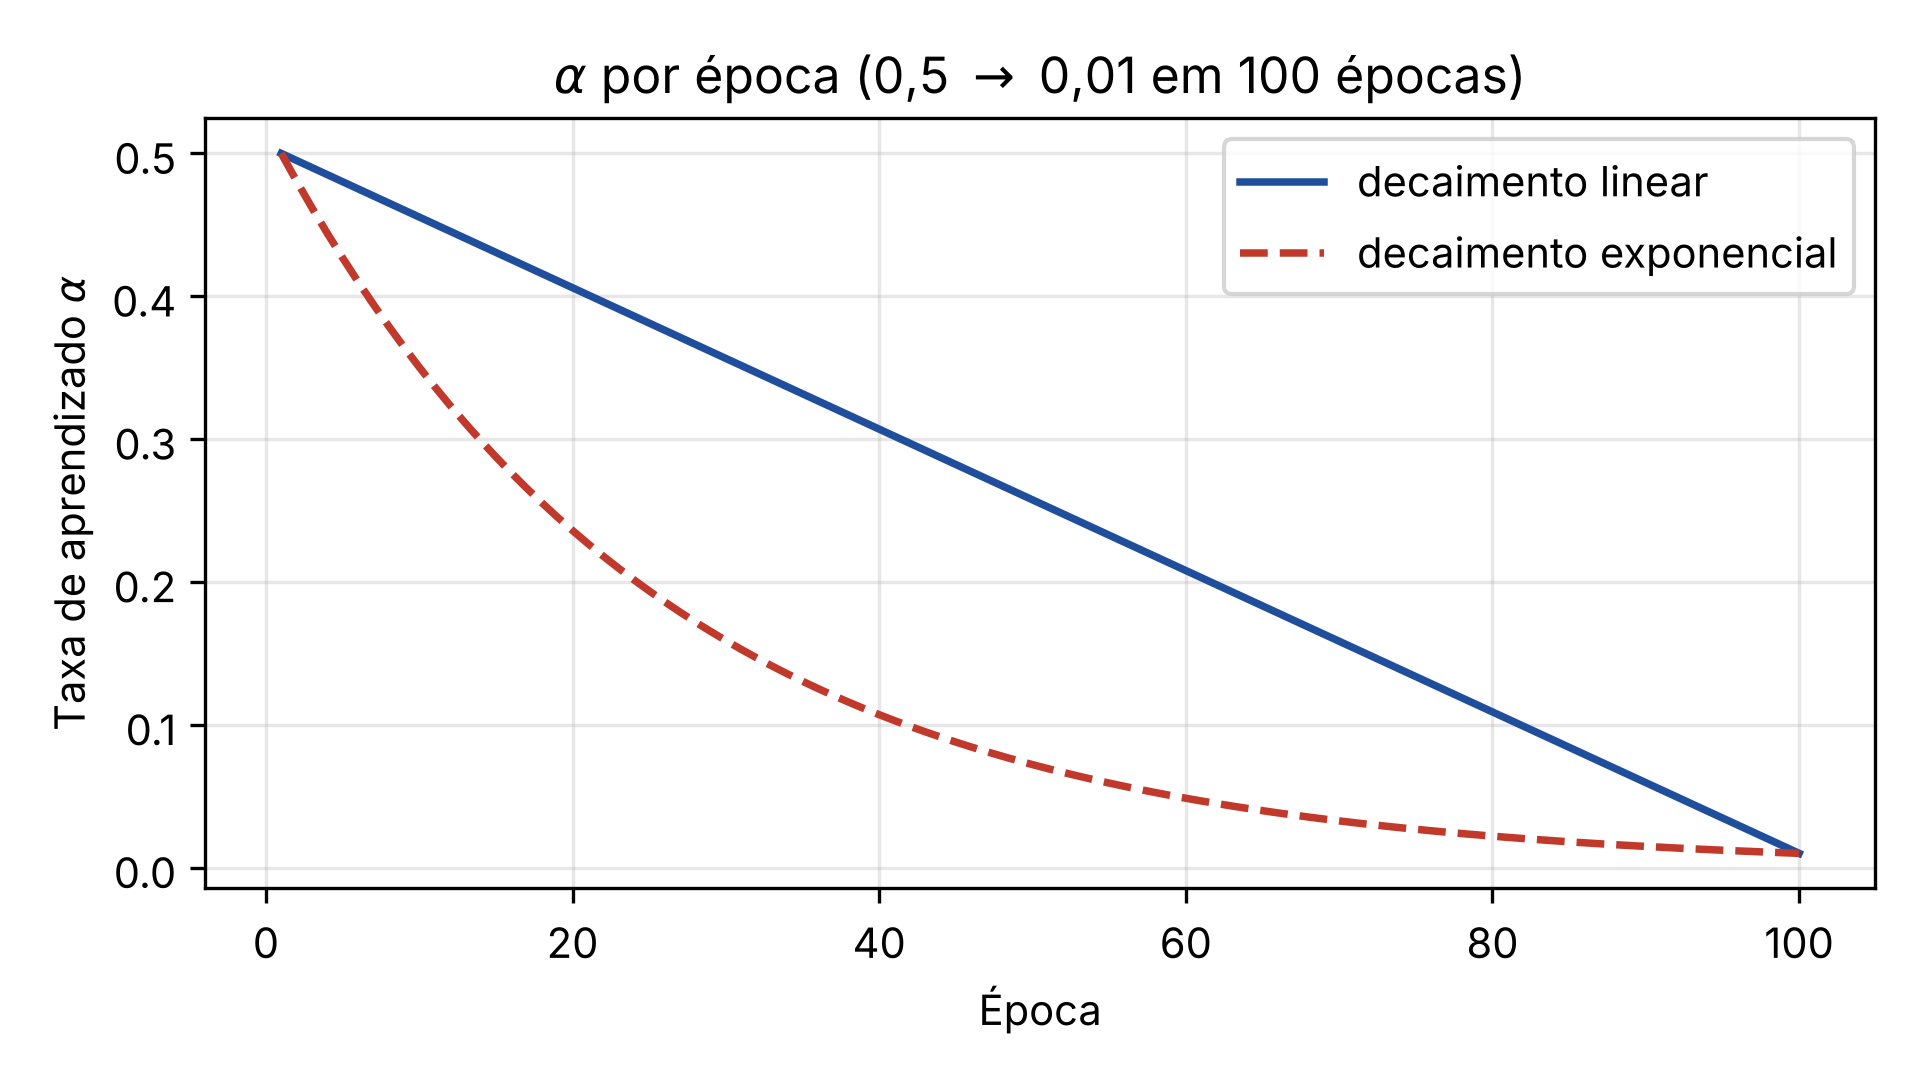
\includegraphics[width=0.72\textwidth]{alpha_por_epoca.png}
  \caption{Taxa de aprendizado em cada época para os decaimentos linear
  (padrão) e exponencial.}
  \label{fig:alfa}
\end{figure}

\subsection{Métricas de acompanhamento}

Além da inspeção visual, três métricas foram calculadas:
\begin{itemize}
  \item \textbf{Erro de quantização médio}:
  $\EQ=\frac{1}{P}\sum_{p=1}^{P}\min_j\|\mathbf{x}_p-\mathbf{w}_{\cdot j}\|$,
  a distância média de cada ponto ao vetor de pesos vencedor;
  \item \textbf{Número de cruzamentos}: quantidade de pares de segmentos não
  adjacentes da poligonal $C_1$--$C_2$--$\cdots$--$C_{50}$ que se
  intersectam. Zero cruzamentos indica uma curva sem ``nós'' no plano;
  \item \textbf{Unidades mortas}: unidades que não vencem para nenhum padrão
  de treino.
\end{itemize}

A implementação (\texttt{som\_kohonen.py}, Apêndice~\ref{ap:codigo}) usa
apenas Python e NumPy no algoritmo e Matplotlib nas figuras. O mesmo
conteúdo está no notebook \texttt{som\_kohonen.ipynb}.

%=====================================================================
\section{Resultados}
%=====================================================================

A Tabela~\ref{tab:evolucao} reproduz a saída do programa a cada 10 épocas, e
a Figura~\ref{fig:painel} mostra a configuração dos 50 vetores de peso nesses
mesmos instantes, sobrepostos aos pontos de treino e ao círculo
$x_1^2+x_2^2=0{,}25$.

\begin{table}[H]
  \centering
  \caption{Evolução do treino principal ($R=1$, decaimento linear,
  semente 42). $\alpha$ é o valor usado na época indicada.}
  \label{tab:evolucao}
  \small
  \begin{tabular}{rccr}
    \toprule
    Época & $\alpha$ & EQ & Cruzamentos \\
    \midrule
      0 & --     & 0,1397 & 209 \\
     10 & 0,4555 & 0,0485 &  15 \\
     20 & 0,4060 & 0,0466 &   4 \\
     30 & 0,3565 & 0,0464 &   4 \\
     40 & 0,3070 & 0,0453 &   4 \\
     50 & 0,2575 & 0,0447 &   4 \\
     60 & 0,2080 & 0,0418 &   4 \\
     70 & 0,1585 & 0,0414 &   4 \\
     80 & 0,1090 & 0,0416 &   4 \\
     90 & 0,0595 & 0,0420 &   4 \\
    100 & 0,0100 & 0,0417 &   4 \\
    \bottomrule
  \end{tabular}
\end{table}

\begin{figure}[H]
  \centering
  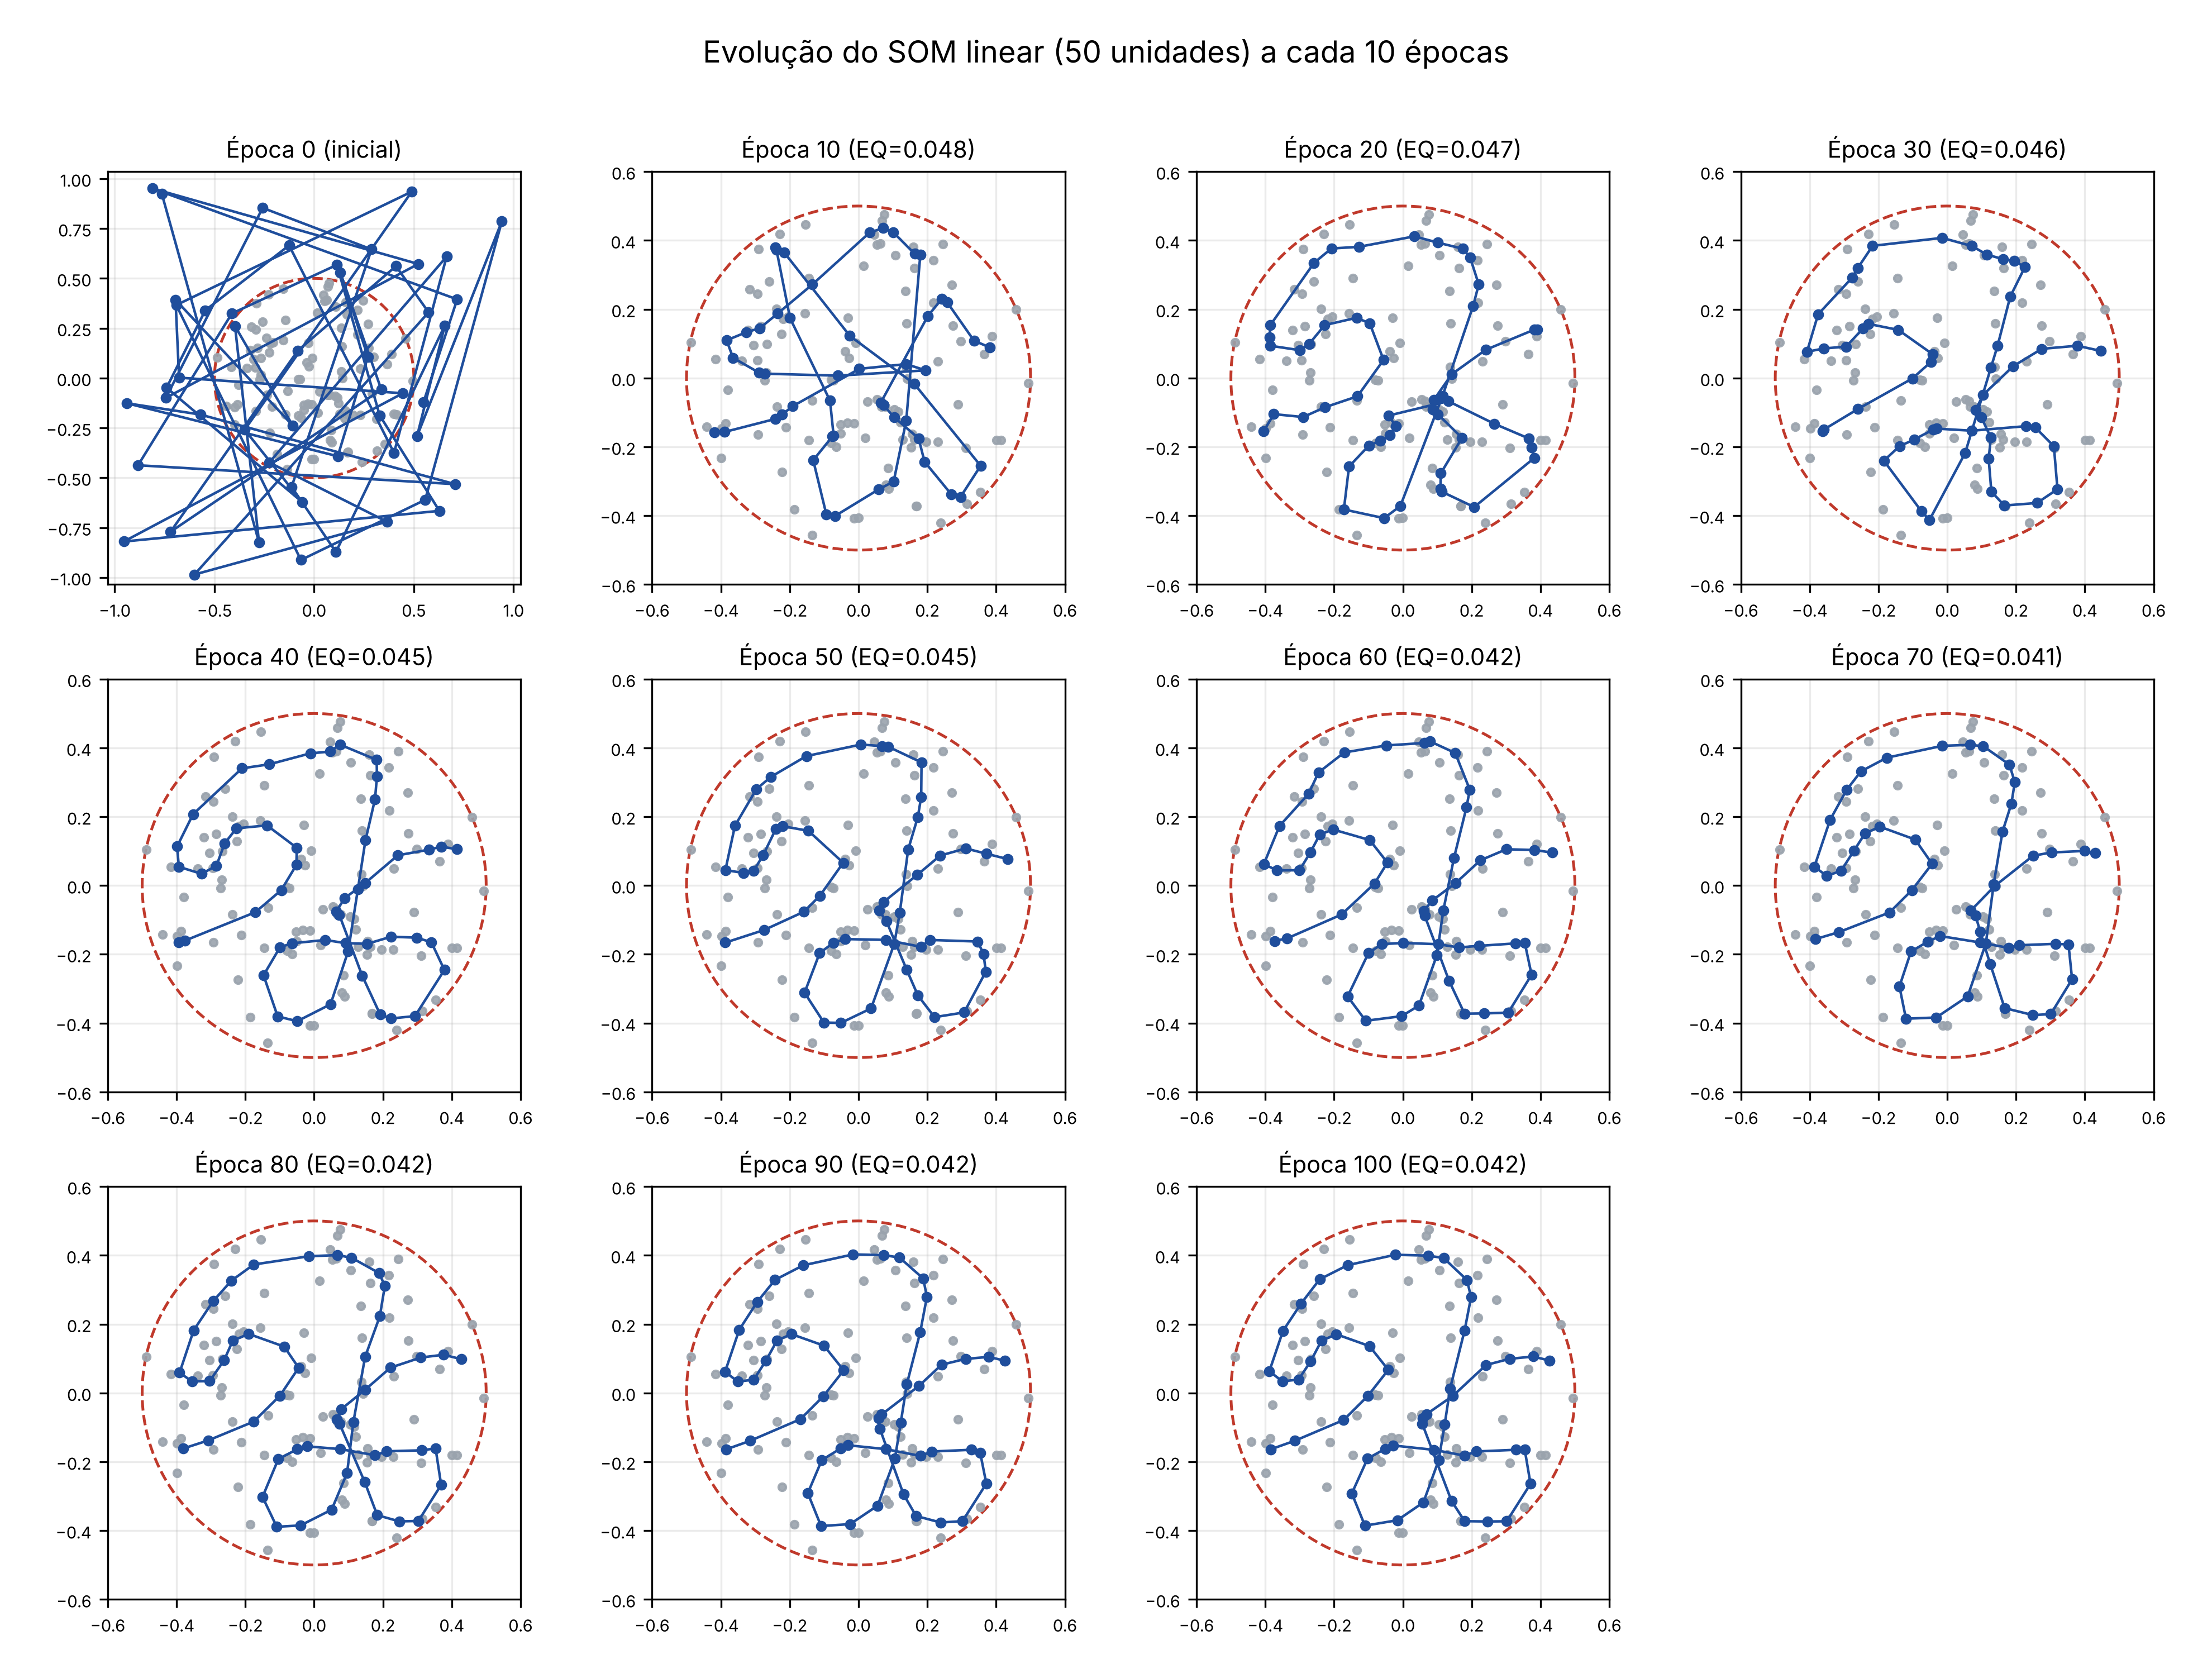
\includegraphics[width=\textwidth]{som_painel.png}
  \caption{Vetores de peso das 50 unidades (pontos azuis ligados na ordem
  $C_1$--$C_{50}$) nas épocas 0, 10, \dots, 100, sobre os dados de treino
  (cinza) e o círculo $x_1^2+x_2^2=0{,}25$ (tracejado). As figuras
  individuais de cada época estão em \texttt{figuras/som\_epoca\_XXX.png}.}
  \label{fig:painel}
\end{figure}

\begin{figure}[H]
  \centering
  \begin{subfigure}{0.49\textwidth}
    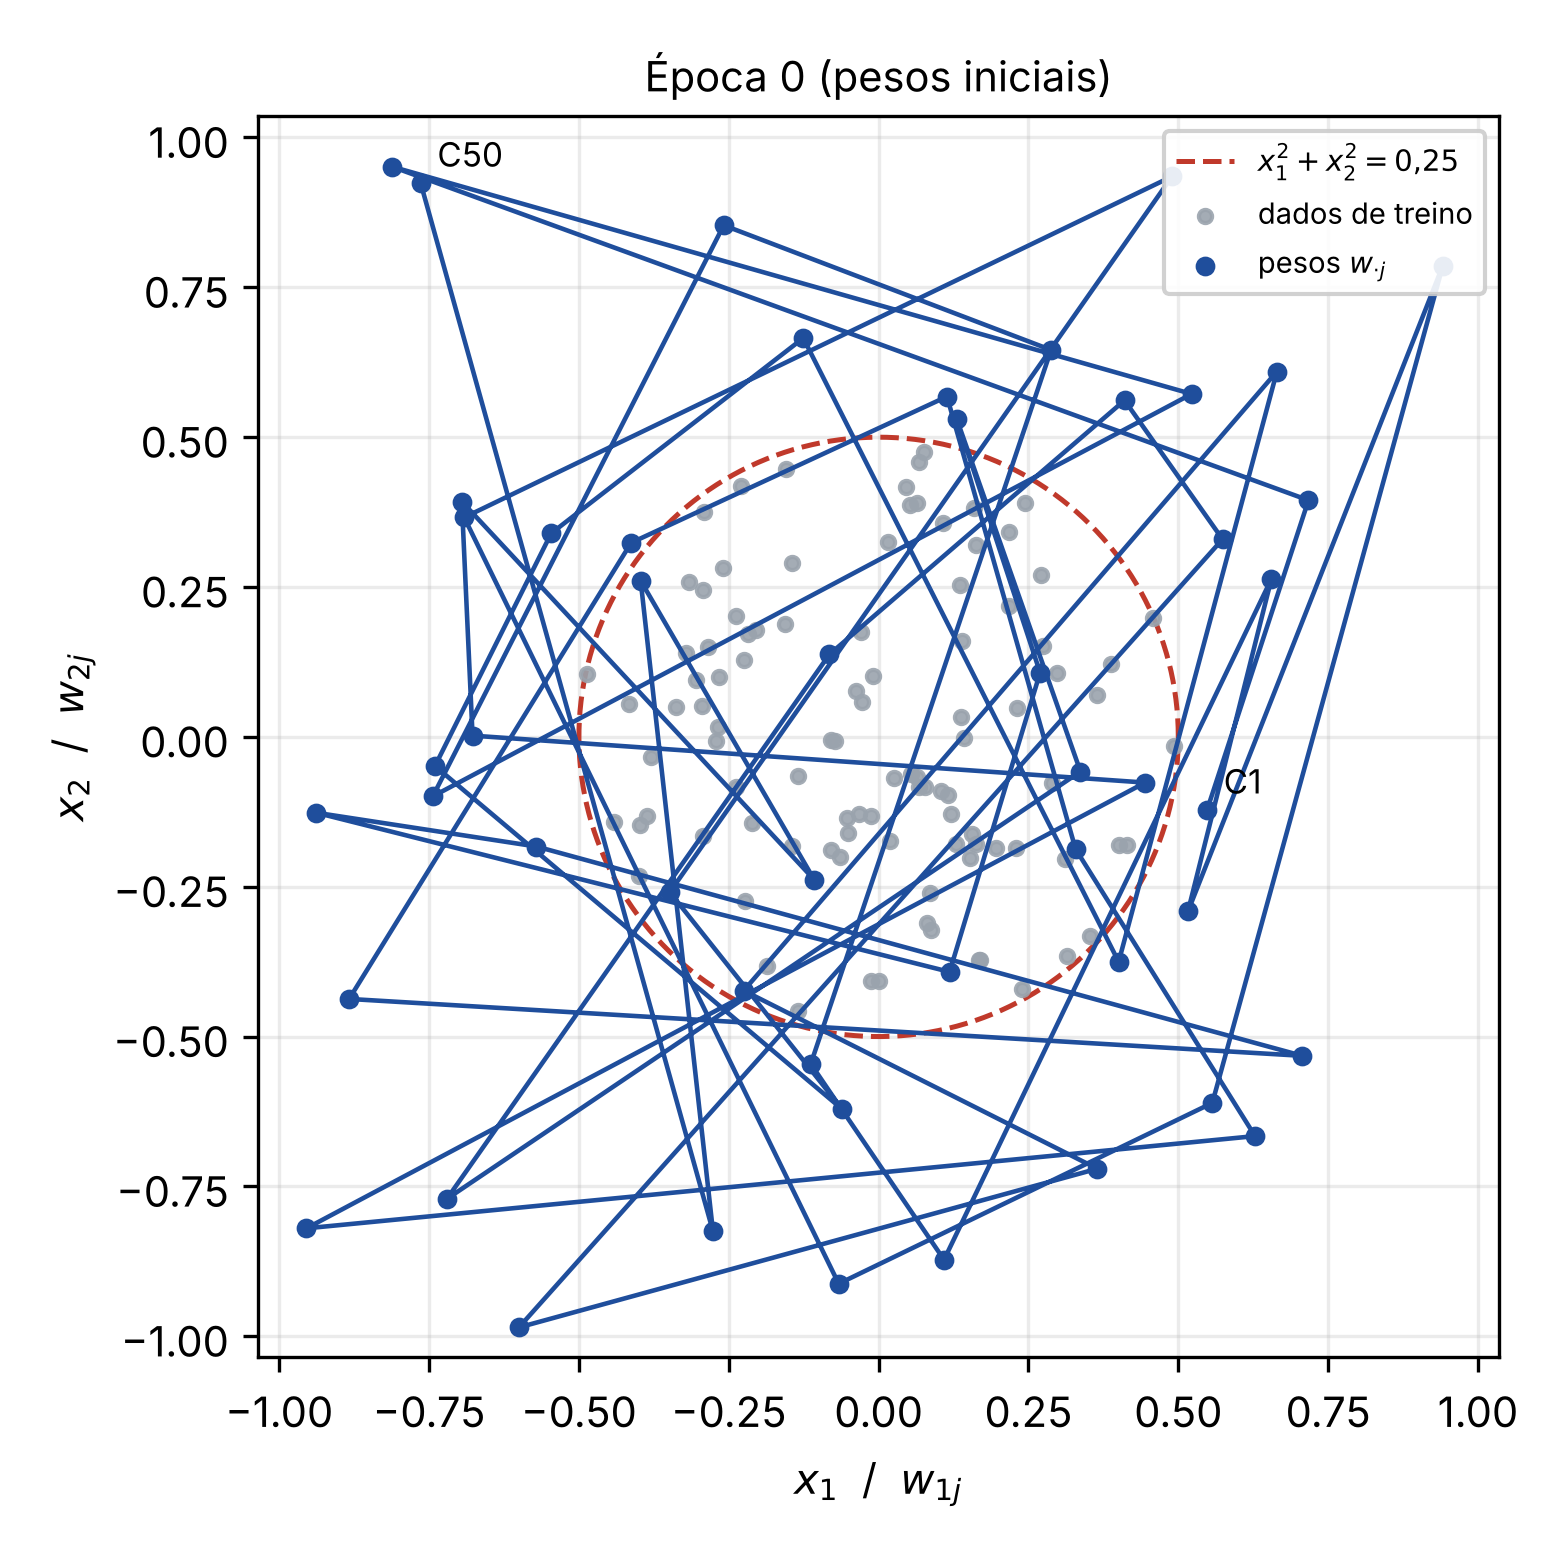
\includegraphics[width=\linewidth]{som_epoca_000.png}
    \caption{Época 0: pesos iniciais em $U(-1,1)^2$.}
  \end{subfigure}\hfill
  \begin{subfigure}{0.49\textwidth}
    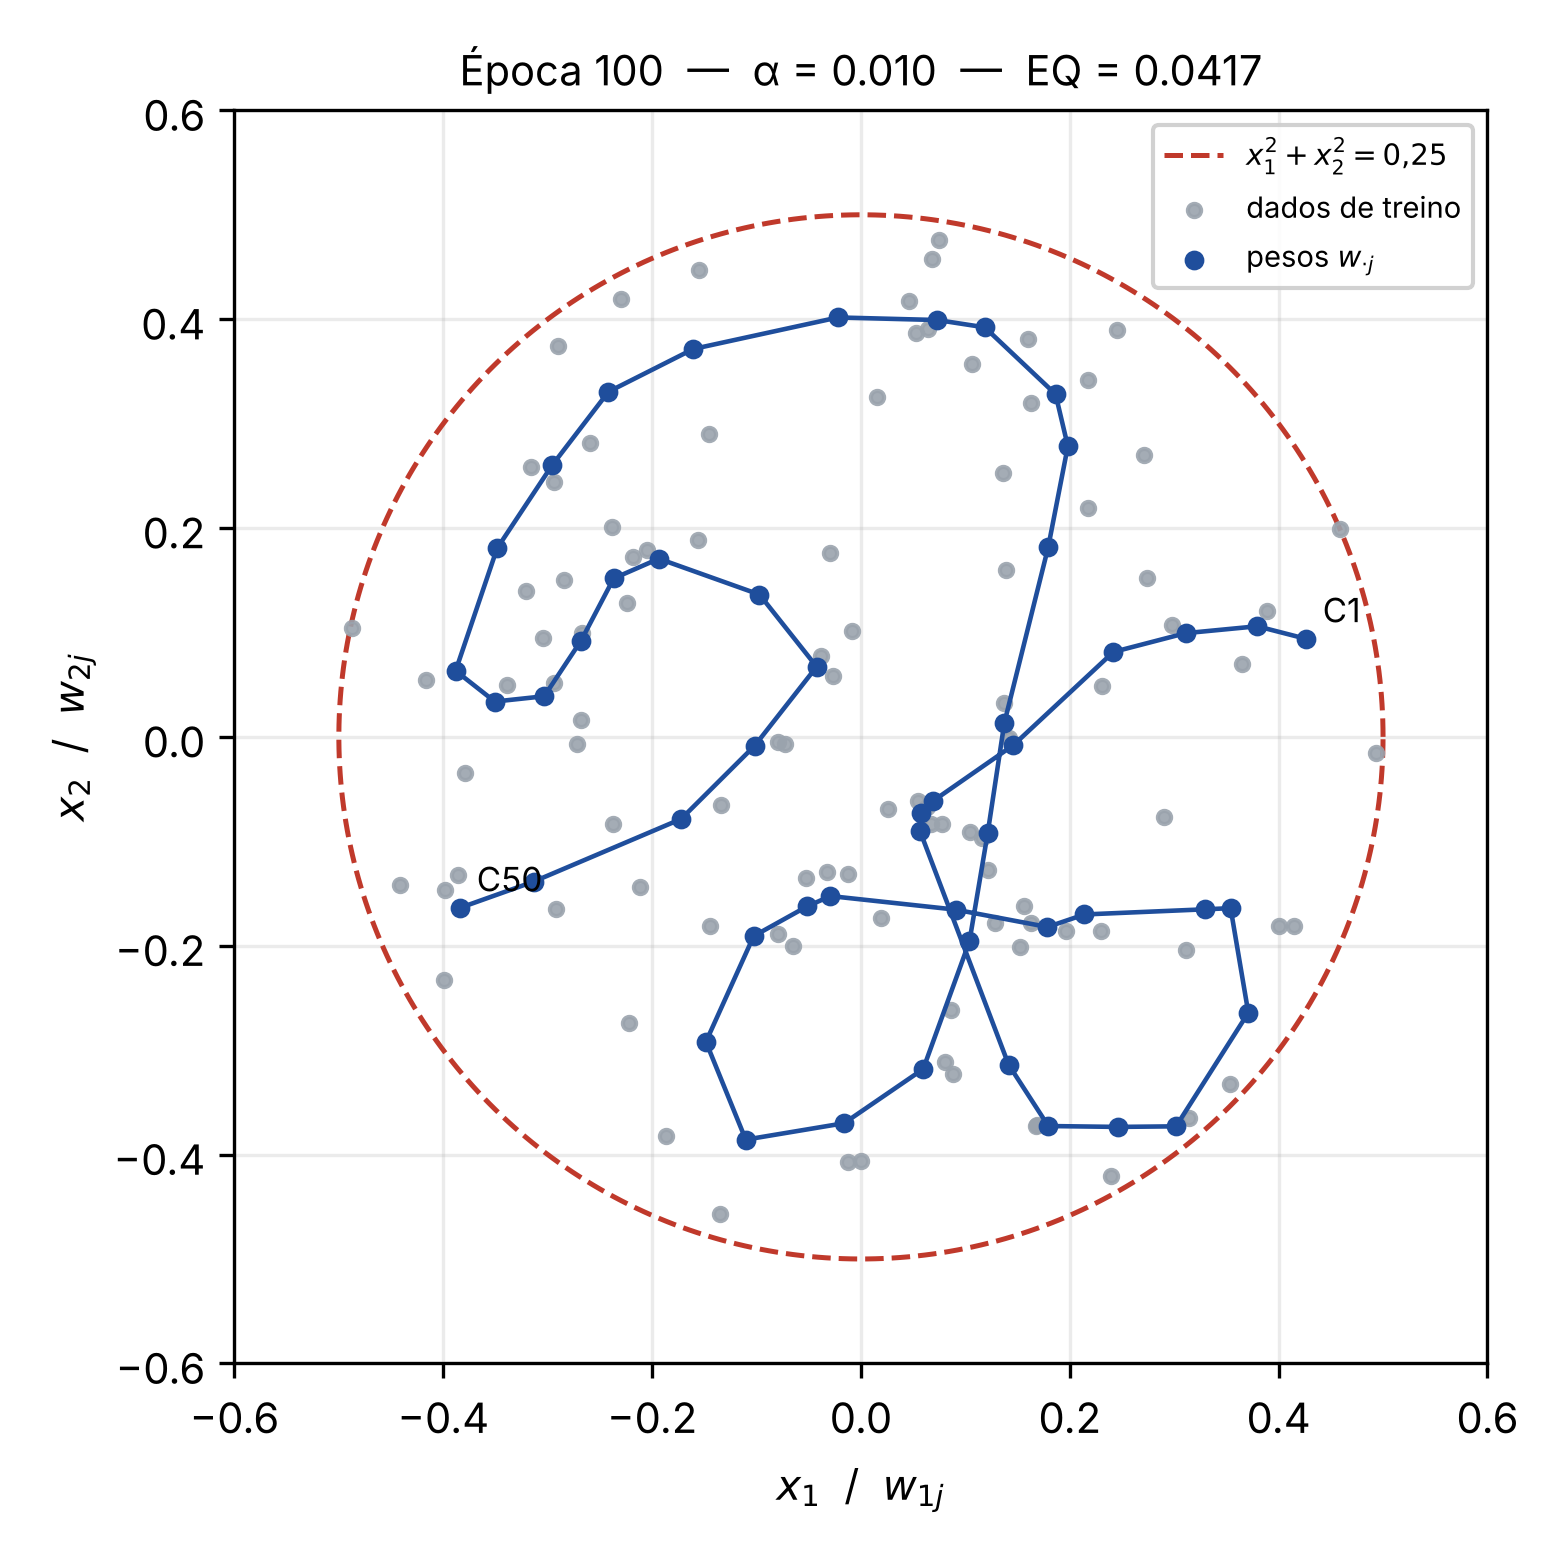
\includegraphics[width=\linewidth]{som_epoca_100.png}
    \caption{Época 100: configuração final.}
  \end{subfigure}
  \caption{Estado inicial e final da rede, em detalhe.}
  \label{fig:inicial-final}
\end{figure}

A evolução tem duas fases nítidas:

\begin{itemize}
  \item \textbf{Ordenação (épocas 1--10).} Na época 0 os pesos estão
  espalhados por todo o quadrado $[-1,1]^2$. Como a maioria fica fora do
  disco, a cadeia atravessa o plano 209 vezes. Com $\alpha\approx0{,}5$, cada
  atualização leva o vencedor e seus dois vizinhos a meio caminho do padrão
  apresentado, e em dez épocas todos os pesos foram puxados para dentro do
  disco. A maior parte do emaranhado se desfaz (de 209 para 15 cruzamentos),
  e o erro de quantização cai quase três vezes, de $0{,}140$ para $0{,}048$.
  \item \textbf{Convergência (épocas 10--100).} A forma global da curva
  praticamente congela. Os cruzamentos caem para 4 até a época 20 e
  permanecem nesse valor até o fim. O que muda é o detalhe local: com
  $\alpha$ decrescendo, os pesos se acomodam nos agrupamentos de pontos,
  os segmentos ficam mais regulares e o EQ desce lentamente até $0{,}042$
  (Figura~\ref{fig:erro}).
\end{itemize}

\begin{figure}[H]
  \centering
  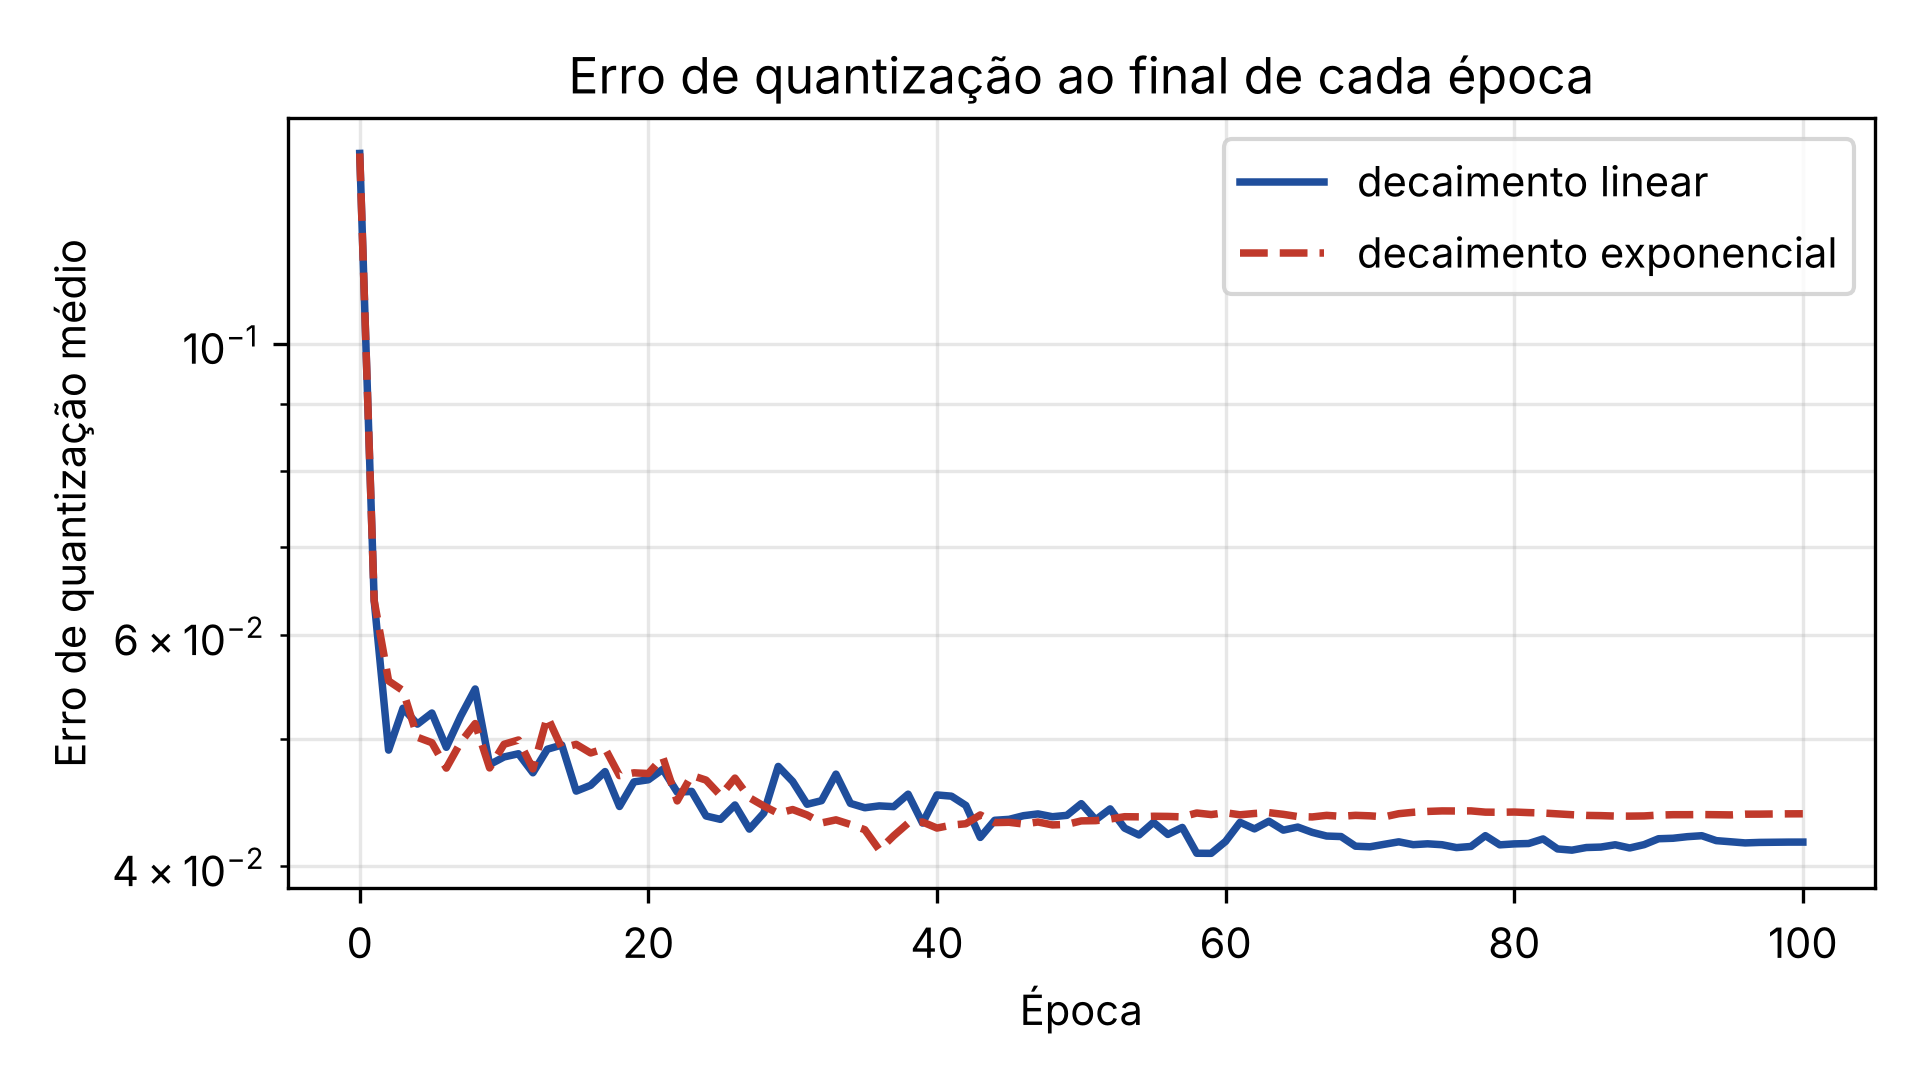
\includegraphics[width=0.72\textwidth]{erro_quantizacao.png}
  \caption{Erro de quantização médio ao final de cada época (escala
  logarítmica) para os dois decaimentos de $\alpha$.}
  \label{fig:erro}
\end{figure}

Ao final, a cadeia tem comprimento total $4{,}31$ e espaçamento médio de
$0{,}088$ entre unidades consecutivas (mínimo de $0{,}016$, máximo de
$0{,}239$). Ela serpenteia por todo o disco, alcançando raio $0{,}48$, mas
mantém 4 cruzamentos concentrados próximos ao centro e ao quadrante inferior
direito (Figura~\ref{fig:inicial-final}b). As unidades extremas $C_1$ e
$C_{50}$ ficam junto à borda do disco.

\subsection{Análises complementares}

\paragraph{Decaimento exponencial.} Com a mesma semente, o decaimento
exponencial leva a uma configuração final de forma semelhante, com 3
cruzamentos e $\EQ=0{,}0439$ (Figura~\ref{fig:comp-decaimento}). Como
$\alpha$ cai mais depressa (já vale $0{,}11$ na época 40), o mapa
``congela'' mais cedo: o EQ quase não muda depois da época 40
(Figura~\ref{fig:erro}).

\begin{figure}[H]
  \centering
  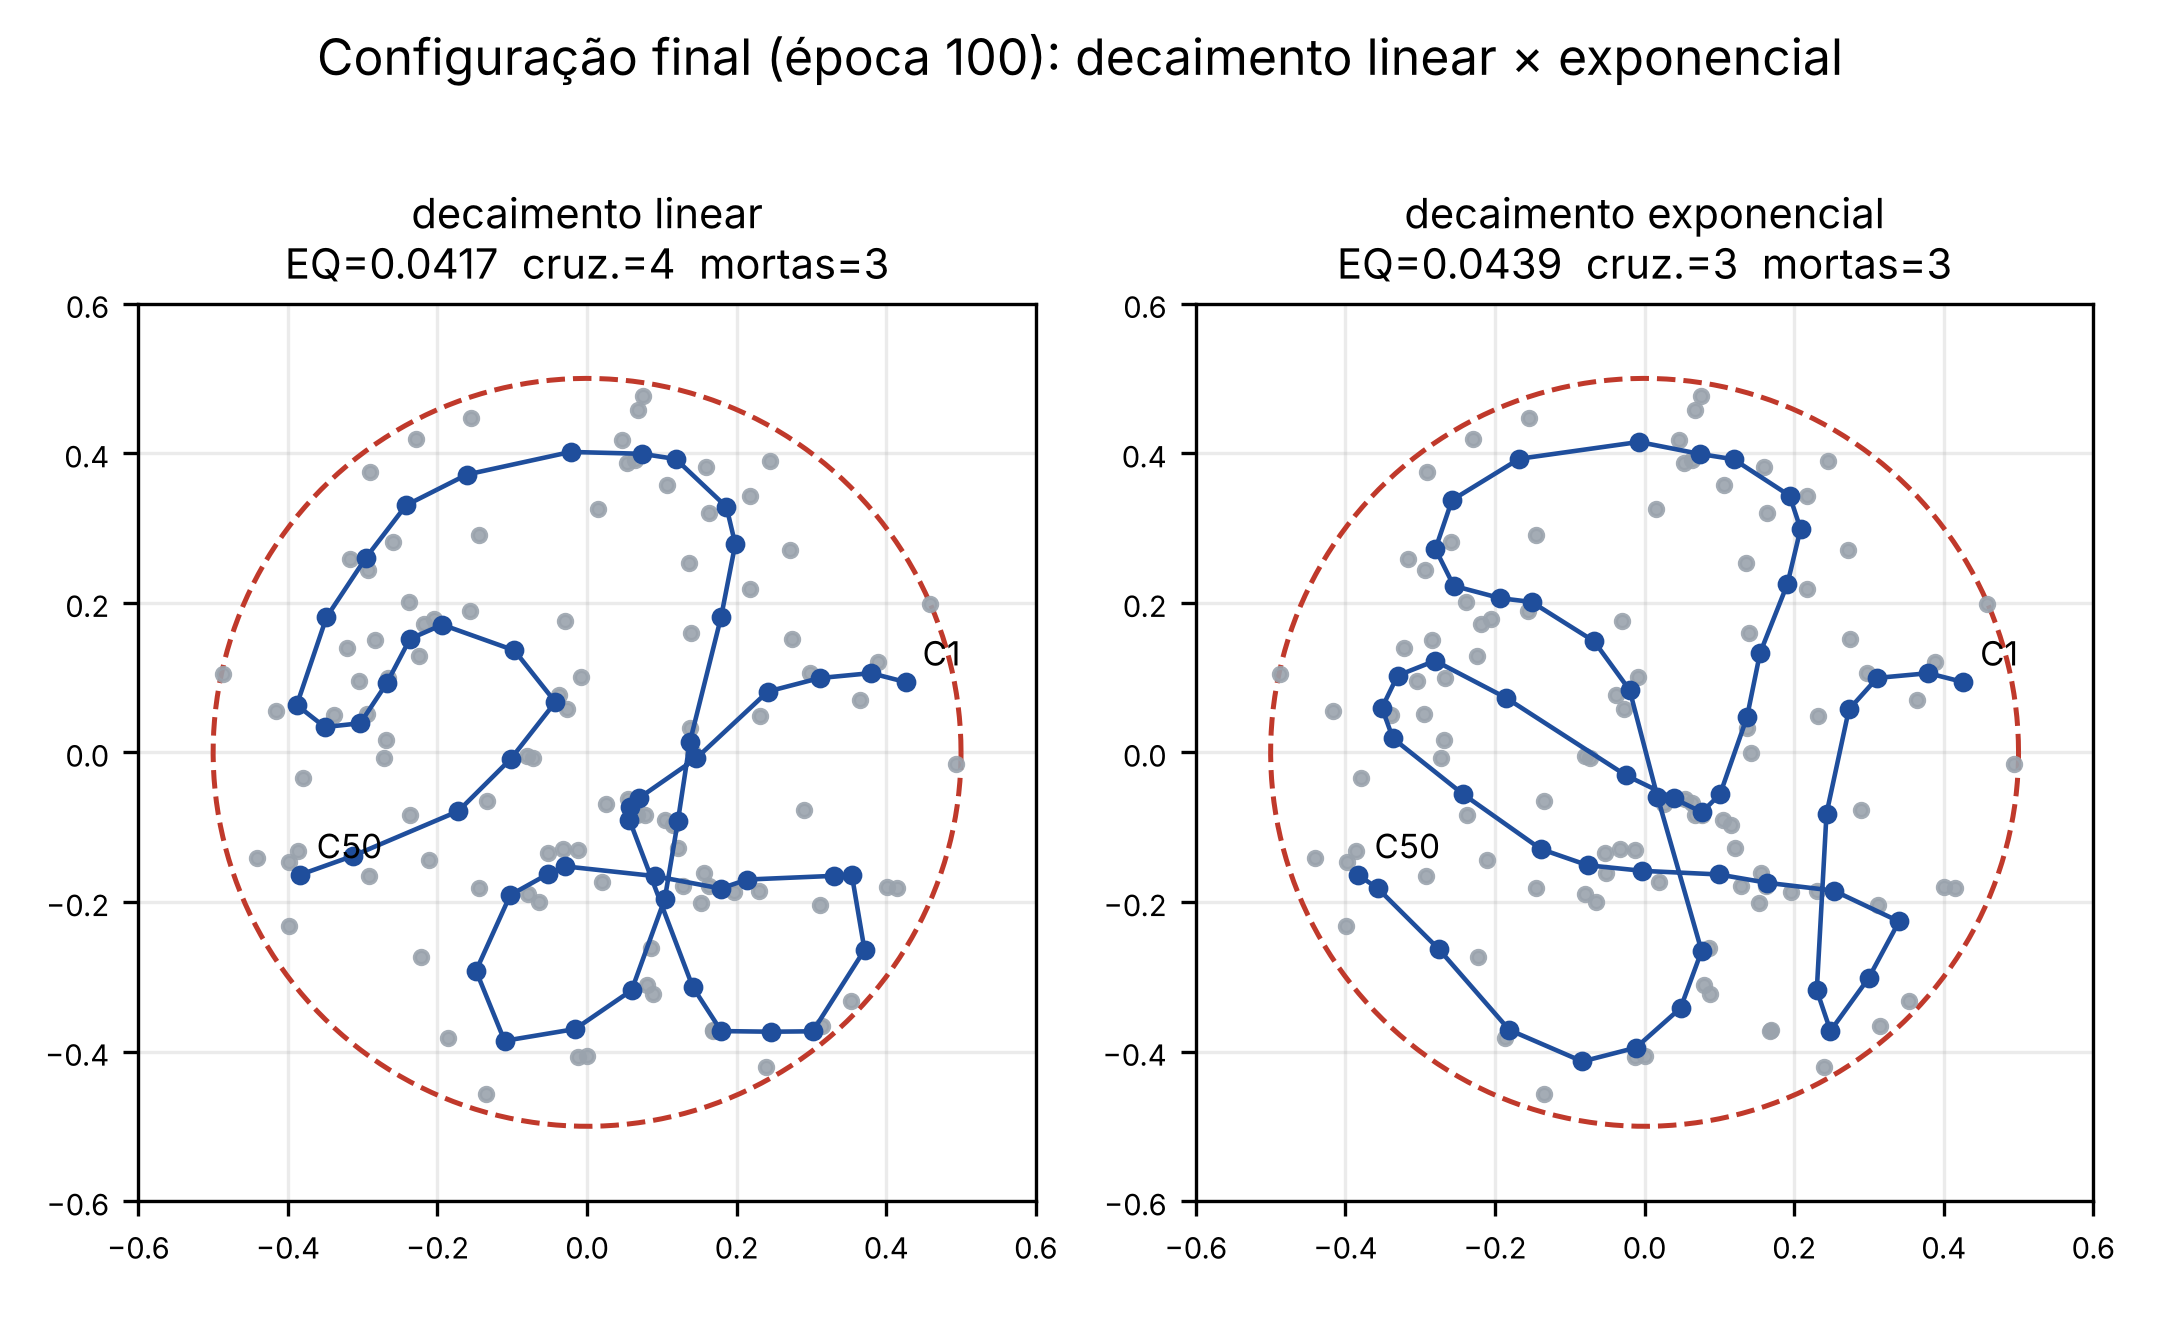
\includegraphics[width=0.78\textwidth]{comparacao_decaimento.png}
  \caption{Configuração final com decaimento linear e exponencial de
  $\alpha$ (mesmos dados e mesma semente).}
  \label{fig:comp-decaimento}
\end{figure}

\paragraph{Sementes diferentes.} Mantidos os dados e o decaimento linear,
variou-se a semente da rede, que define os pesos iniciais e a ordem de
apresentação. A Tabela~\ref{tab:seeds} e a Figura~\ref{fig:comp-seeds}
mostram que o EQ final é estável, entre $0{,}040$ e $0{,}043$, mas a
quantidade de nós residuais varia de 0 a 4. A semente 1 produziu uma curva
sem cruzamentos.

\begin{table}[H]
  \centering
  \caption{Resultado final (época 100) para diferentes sementes da rede.}
  \label{tab:seeds}
  \small
  \begin{tabular}{rcccc}
    \toprule
    Semente & EQ & Cruzamentos & Unidades mortas & Comprimento da cadeia \\
    \midrule
       42 & 0,0417 & 4 & 3 & 4,31 \\
        1 & 0,0426 & 0 & 4 & 3,88 \\
        7 & 0,0431 & 4 & 2 & 4,57 \\
     2024 & 0,0397 & 2 & 1 & 4,35 \\
    31415 & 0,0421 & 2 & 2 & 4,11 \\
    \bottomrule
  \end{tabular}
\end{table}

\begin{figure}[H]
  \centering
  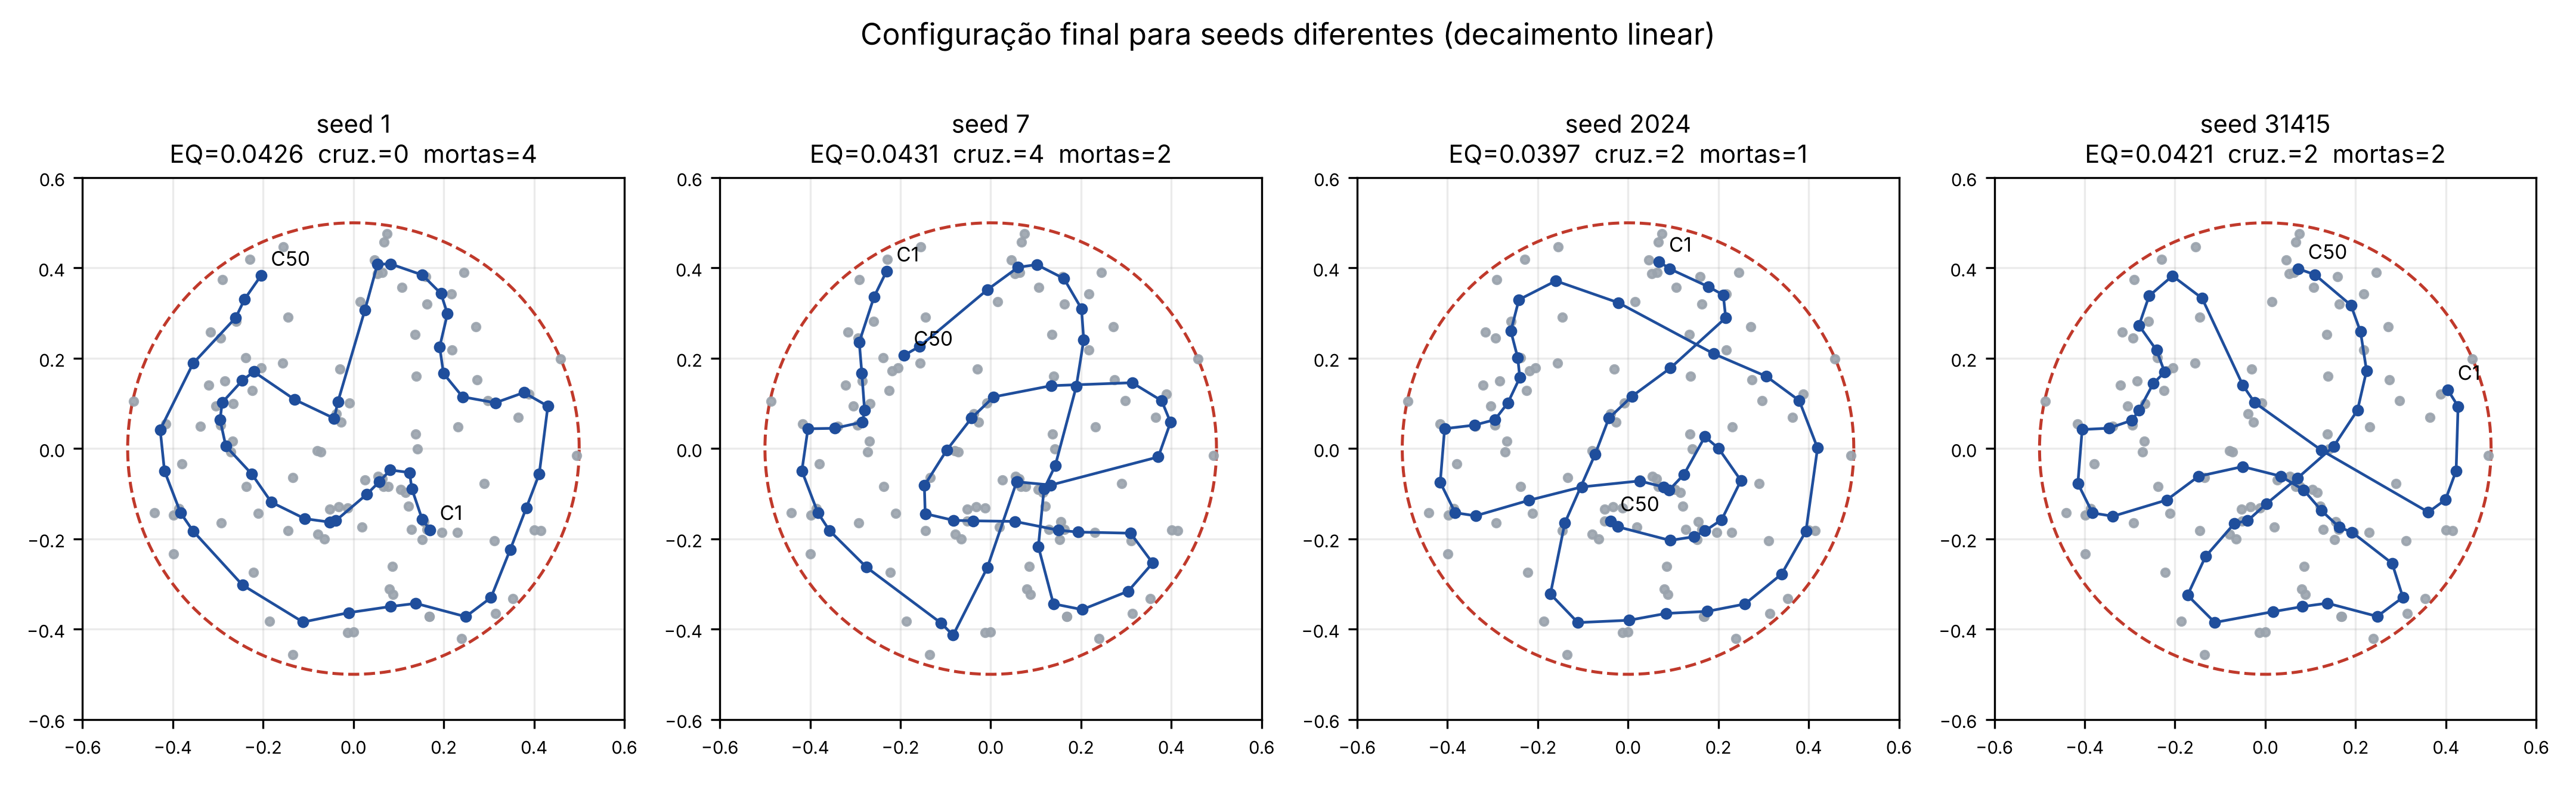
\includegraphics[width=\textwidth]{comparacao_seeds.png}
  \caption{Configuração final para quatro sementes adicionais.}
  \label{fig:comp-seeds}
\end{figure}

\paragraph{Raio decrescente (fora do enunciado).} Para isolar o papel da
vizinhança, repetiu-se o treino com a mesma semente, mas com raio inicial
$R=10$, reduzido linearmente até $R=1$ na época 50 e mantido em 1 depois
disso. A cadeia fica sem nenhum cruzamento já na época 10 e termina
desembaraçada, com $\EQ=0{,}0401$ e apenas uma unidade morta
(Figura~\ref{fig:comp-raio}). O preço é um EQ maior durante a fase de raio
grande (0,108 na época 10, contra 0,048 com $R=1$), porque cada atualização
arrasta muitas unidades ao mesmo tempo e a cadeia fica ``tensionada''.

\begin{figure}[H]
  \centering
  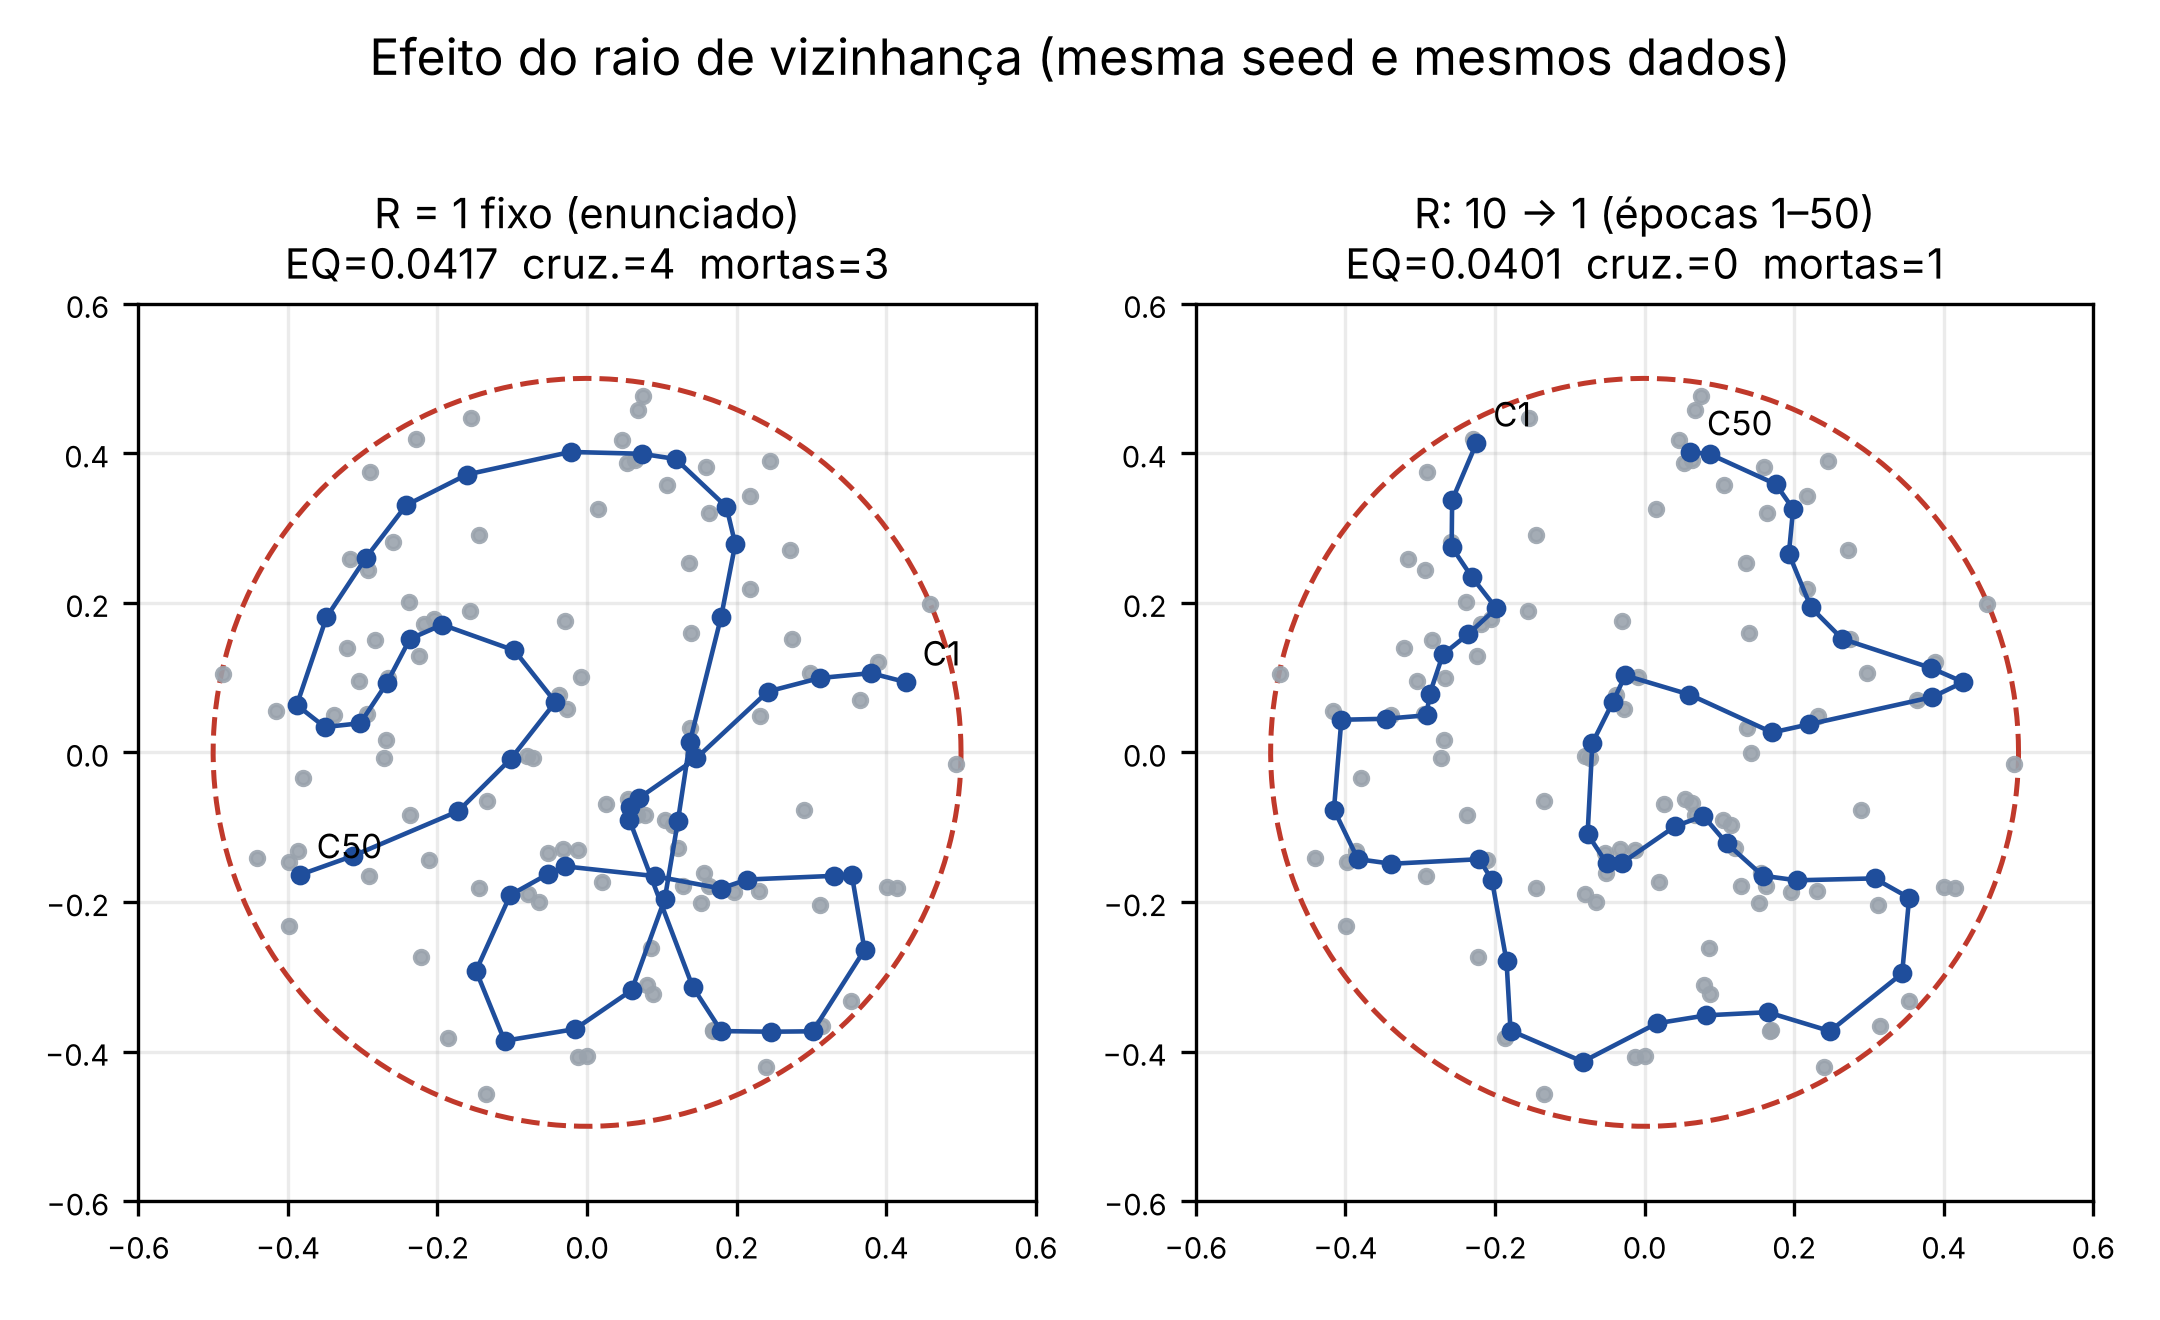
\includegraphics[width=0.78\textwidth]{comparacao_raio.png}
  \caption{Efeito do raio de vizinhança: $R=1$ fixo (enunciado) e $R$
  decrescente de 10 a 1 (mesmos dados e mesma semente).}
  \label{fig:comp-raio}
\end{figure}

%=====================================================================
\section{Discussão}
%=====================================================================

\paragraph{Efeito da vizinhança $R=1$.} A vizinhança é o que transforma o
aprendizado competitivo em mapa topológico. Com $R=1$, cada atualização
acopla apenas três unidades, então a ordem da cadeia só se propaga por
contato entre vizinhos imediatos. Isso basta para desfazer cruzamentos
\emph{locais}. Um ``nó'' formado entre trechos distantes da cadeia, porém,
exigiria que dezenas de unidades se movessem de forma coordenada, e nenhuma
atualização isolada produz esse movimento. Na prática, a configuração global
fica decidida nas primeiras épocas e depende da inicialização (Tabela~\ref{tab:seeds}).
O experimento com raio decrescente confirma o diagnóstico. É por isso que
Kohonen (2001) e Haykin (2001) recomendam começar com uma
vizinhança que abranja boa parte da rede e reduzi-la gradualmente. O
exercício, ao fixar $R=1$, evidencia justamente o que se perde sem essa fase.

\paragraph{Efeito do decaimento de $\alpha$.} Um $\alpha$ alto no início
permite grandes deslocamentos e acelera a ordenação. Um $\alpha$ pequeno no
fim faz cada peso convergir para uma média local dos padrões que ele vence,
o que reduz o EQ e estabiliza o mapa. Os dois decaimentos testados terminam
em configurações equivalentes. O linear mantém a rede plástica por mais
tempo, e o exponencial congela o mapa antes. Com $R=1$ fixo, porém, mais
plasticidade não basta para desfazer os nós globais. A ordenação depende
mais do raio do que de $\alpha$.

\paragraph{Densidade de unidades e densidade dos dados.} Há 50 unidades para
100 pontos, cerca de dois pontos por unidade. Na rede principal, 13 unidades
vencem um único ponto, 19 vencem dois, 12 vencem três e o máximo é cinco.
Três unidades não vencem nenhum ponto. Unidades mortas como essas não
são desperdício puro: ficam entre unidades ativas e funcionam como
``elos'' de interpolação: a restrição topológica obriga a curva a passar por
ali. A distribuição radial dos pesos acompanha a dos dados. A fração de
pesos com $\|\mathbf{w}\|<0{,}25$ é $0{,}30$, contra $0{,}31$ dos pontos,
e os raios médios são $0{,}298$ e $0{,}306$. Isso indica que a rede aloca
unidades aproximadamente na proporção da densidade, como esperado para
um SOM (KOHONEN, 2001). Com apenas 100 amostras, a densidade ``vista'' pela
rede não é uniforme, e flutuações locais (aglomerados e vazios) explicam a
variação no espaçamento entre unidades.

\paragraph{Dobras e nós residuais.} Para preencher um disco, uma curva
unidimensional precisa se dobrar, e as dobras em ``U'' observadas são
inerentes ao problema, não defeitos. Defeitos são os cruzamentos, em que dois
trechos distantes da cadeia representam regiões sobrepostas. Nesses pontos a
preservação topológica é violada localmente: unidades distantes na cadeia
ficam próximas no plano. Também se observa o efeito de borda: as unidades
extremas têm um só vizinho, são menos ``puxadas'' e tendem a se fixar na
periferia do disco.

%=====================================================================
\section{Conclusão}
%=====================================================================

A rede de Kohonen linear do Exercício 4.1 foi implementada e treinada
conforme o enunciado. Os resultados mostram o comportamento esperado de um
SOM. Em cerca de dez épocas o emaranhado aleatório se recolhe para o disco e
se ordena em uma curva que serpenteia pela região dos dados. Depois disso, a
redução de $\alpha$ refina a quantização, levando o EQ de $0{,}140$ a
$0{,}042$. A distribuição das unidades acompanha a dos dados.

O raio fixo $R=1$ limita a ordenação global. A maioria das execuções
termina com alguns nós residuais, cuja quantidade depende da inicialização.
O decaimento de $\alpha$, linear ou exponencial, tem efeito secundário,
enquanto uma vizinhança inicial ampla elimina os nós por completo. Esses
resultados reforçam o papel central da cooperação entre vizinhos na
auto-organização. Uma extensão natural seria medir a frequência de nós em
muitas sementes e avaliar métricas formais de preservação topológica, como o
erro topográfico.

%=====================================================================
\renewcommand{\refname}{Referências}
\begin{thebibliography}{9}
\makeatletter\renewcommand\@biblabel[1]{}\makeatother
\setlength{\itemindent}{-\leftmargin}\singlespacing
%=====================================================================
\bibitem{fausett}
FAUSETT, L. \textbf{Fundamentals of neural networks}: architectures,
algorithms, and applications. Englewood Cliffs: Prentice Hall, 1994.

\bibitem{haykin}
HAYKIN, S. \textbf{Redes neurais}: princípios e prática. 2. ed. Porto
Alegre: Bookman, 2001.

\bibitem{kohonen1982}
KOHONEN, T. Self-organized formation of topologically correct feature maps.
\textbf{Biological Cybernetics}, v. 43, n. 1, p. 59--69, 1982.

\bibitem{kohonen2001}
KOHONEN, T. \textbf{Self-organizing maps}. 3. ed. Berlin: Springer, 2001.
\end{thebibliography}

%=====================================================================
\appendix
\section{Código-fonte}
\label{ap:codigo}
%=====================================================================
\lstinputlisting{som_kohonen.py}

\end{document}
